\documentclass{article}
\usepackage{graphicx} % Required for inserting images
\usepackage{amsmath}
\usepackage{float}
\title{Lesson 22 Homework - Proof Writing}
\author{William Wang}
\date{February 2026}

\begin{document}

\maketitle

\section{}

Let 
\[A = (-1,2,4), B = (3,-1,2), C = (5,1,6)\]
Then we can find two direction vectors through these points. 
\[\vec{AB} = \langle 4,-3,-2 \rangle, \vec{AC} = \langle 6,-1,2 \rangle\]
Then we can find the cross product between the two vectors to find the normal vector. 
\[\vec{n} = \vec{AB} \times \vec{BC} = \langle-6-2, -8-12, 8+6 \rangle = \langle -8, -20, 14\rangle\]
Then we have the equation of the plane: 
\[-8(x +1) -20(y-2) + 14(z-4) = 0 \implies -20x-8y+14z = 24\]
Then to find $x$ we can just substitute the points in. 
\[-20x-8(7)+14(10)=24 \implies x = 3\]
\section{}
Let 
\[A = (5,4,1), B = (11,1,-8), C = (5,-1,2), D = (0,14,7)\]
Then we have two direction vectors
\[\vec{AB} = \langle 6,-3,-9 \rangle, \vec{CD} = \langle 5,-15,-5\rangle\]
Then we can find the normal vector by taking the cross product. 
\[\vec{n} = \langle 15-135, -45+30, -90+15\rangle = \langle -120, -15,-75 \rangle = \langle -8, -1, -5 \rangle\]
Then we have the equation of the plane
\[-8(x-5)-(y-4)-5(z-1) = 0 \implies 8x+y+5z = 49\]
\section{}
\begin{figure}[H]
    \centering
    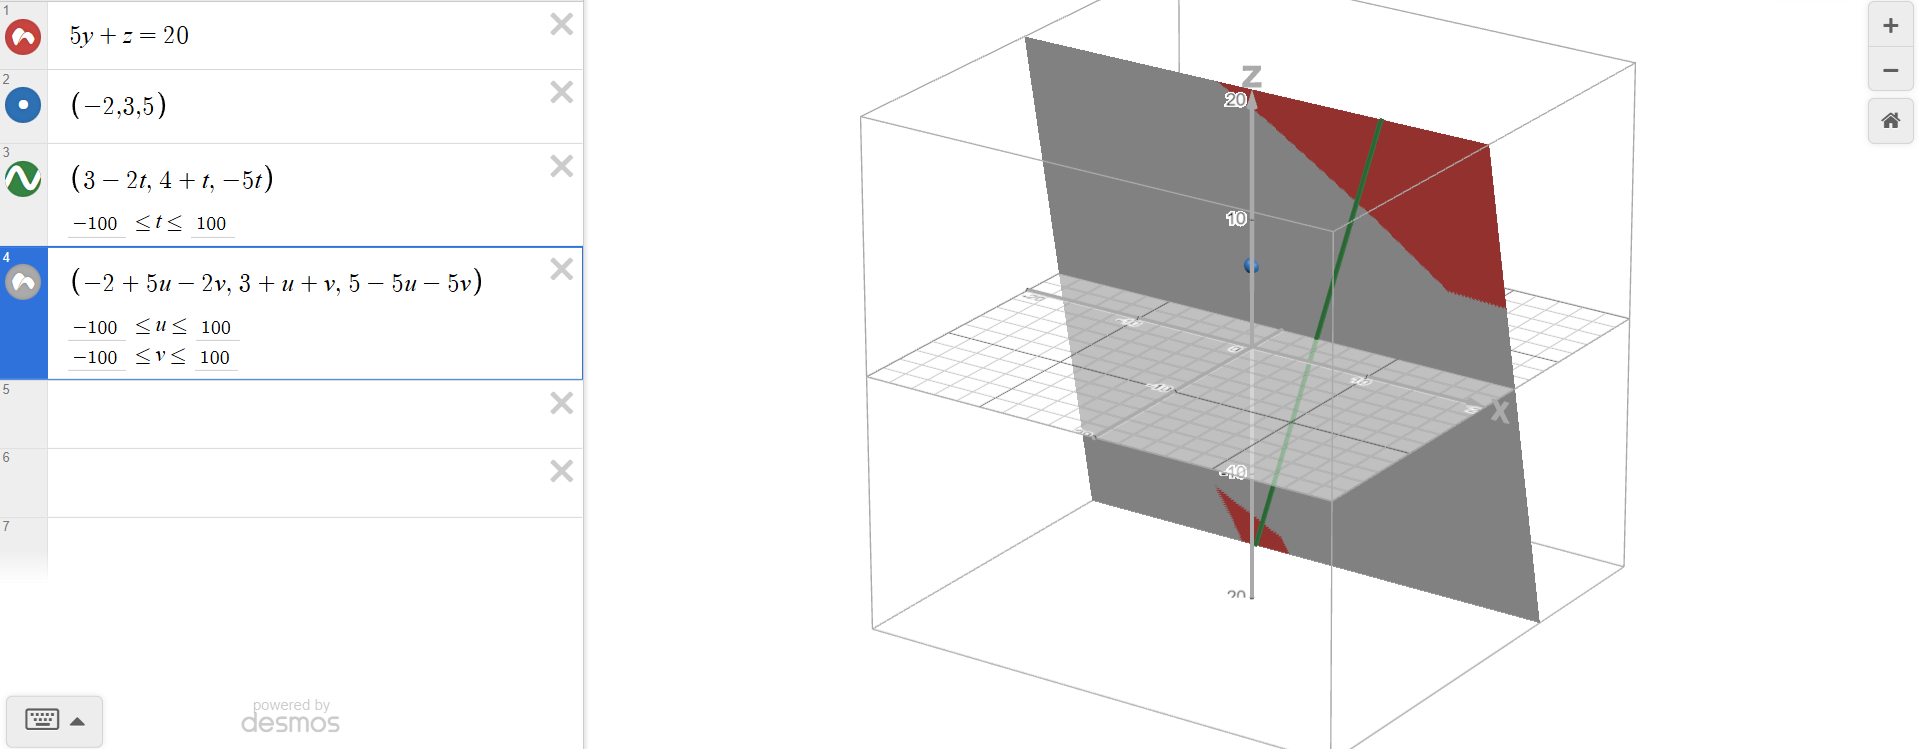
\includegraphics[width=1\linewidth]{q3.png}
\end{figure}
Let \(P = (-2,3,5)\). From the parametric equations, we can find a point and a direction vector. 
\[x = 3-2t\]
\[y = 4+t\]
\[z = -5t\]
From the line we get point \(Q = (3,4,0)\) and a direction vector \(\vec{v} = \langle -2,1,-5 \rangle\). Then we can find the second direction vector. 
\[\vec{w} = \langle5,1,-5 \rangle\]
Then we can find the normal vector
\[\vec{n} = \vec{w} \times \vec{v} = \langle 0, 5, 1 \rangle \]
Hence we can find the equation of the plane. 
\[5(y-3) + (z-5)=0 \implies 5y +z =20\]
Then we can get the parametrization. 
\[\vec{r}(s,t) = P + s\vec{u} + t\vec{v} = (-2,3,5)+s(5,1,-5) + t(-2,1,5)\]
\[x = -2 + 5s -2t\]
\[y = 3+s+t\]
\[z = 5-5s-5t\]


\end{document}
